\begin{figure}[H]
\centering
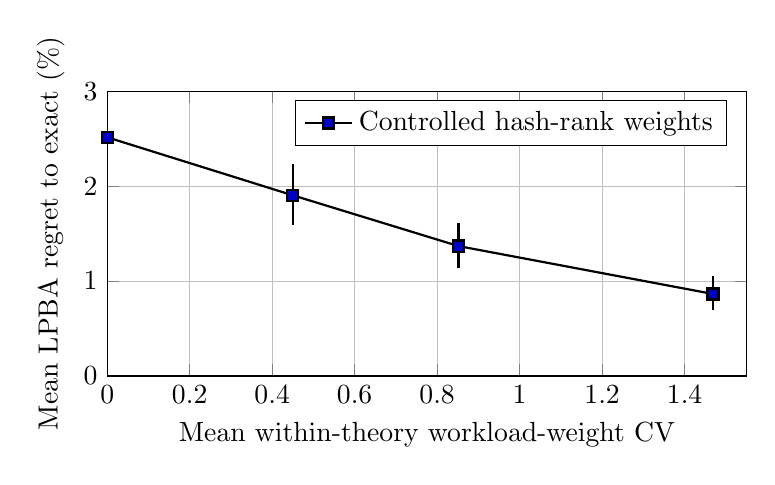
\begin{tikzpicture}
\begin{axis}[width=0.80\textwidth,height=5.2cm,xlabel={Mean within-theory workload-weight CV},ylabel={Mean LPBA regret to exact (\%)},xmin=0,xmax=1.55,ymin=0,ymax=3.0,grid=major,legend pos=north east]
\addplot+[black,mark=square*,thick] coordinates {(0.000,2.514) (0.450,1.903) (0.852,1.368) (1.469,0.864)};
\addlegendentry{Controlled hash-rank weights}
\draw[black,thick] (axis cs:0.000,2.063) -- (axis cs:0.000,3.000);
\draw[black,thick] (axis cs:0.450,1.594) -- (axis cs:0.450,2.232);
\draw[black,thick] (axis cs:0.852,1.137) -- (axis cs:0.852,1.609);
\draw[black,thick] (axis cs:1.469,0.694) -- (axis cs:1.469,1.050);
\end{axis}
\end{tikzpicture}
\caption{Post-hoc sensitivity on the same structural-stress support graphs; vertical bars show theory-bootstrap 95\% intervals. Nonzero settings average three fixed hash seeds per theory. This is synthetic demand, not observed traffic.\label{fig:skew}}
\end{figure}
